\section{Introducción}

Esta es la \textbf{Parte~2} del laboratorio: visión por computadora aplicada al control de
calidad. Se reutiliza el dataset de tapitas de la Parte~1, pero ahora el modelo se entrena
con \emph{aprendizaje por transferencia} (MobileNetV2) y el resultado se envía a un IPC
\textbf{Beckhoff} por el protocolo \textbf{ADS} para accionar un brazo robótico.

\textbf{Materiales.} Los notebooks \texttt{notebook4\_transfer\_learning.ipynb},
\texttt{notebook5\_probar\_modelo.ipynb} y \texttt{notebook6\_envio\_beckhoff.ipynb}; la
librería \texttt{pyads}; y un proyecto TwinCAT con el IPC Beckhoff.

\section{Aprendizaje por transferencia}\label{sec:tl-concepto}

En lugar de entrenar una red desde cero, el \emph{transfer learning} parte de un modelo ya
entrenado sobre millones de imágenes (\textbf{MobileNetV2}, sobre ImageNet) y reutiliza los
filtros que este aprendió. Se procede en dos fases (Figura~\ref{fig:transfer}):

\begin{itemize}
  \item \textbf{Feature extraction}: se \emph{congela} el \emph{backbone} preentrenado y se
        entrena solo un cabezal nuevo (capa densa \emph{softmax}) para las clases del
        problema. Pocas épocas bastan.
  \item \textbf{Fine-tuning}: se \emph{descongelan} las últimas capas del \emph{backbone} y
        se reentrena con un \emph{learning rate} pequeño, para afinar las características de
        alto nivel al dominio de las tapitas sin destruir lo aprendido.
\end{itemize}

La ventaja es decisiva: se obtienen clasificadores robustos con apenas unos cientos de
imágenes por clase, donde una CNN desde cero necesitaría miles.

\begin{figure}[h]
\centering
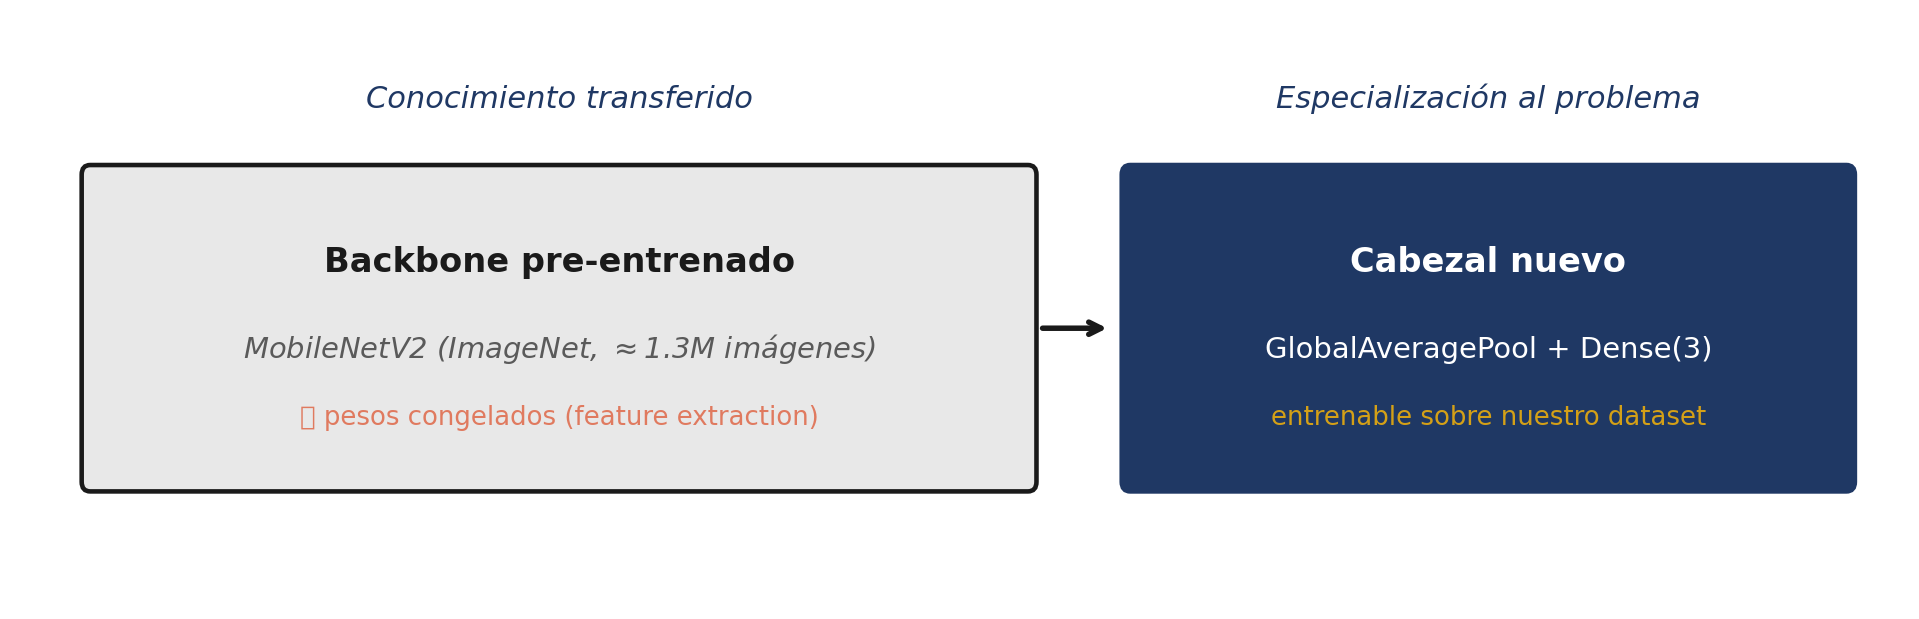
\includegraphics[width=0.95\textwidth]{../docs/assets/g2/transfer_learning.png}
\caption{Aprendizaje por transferencia: se reutiliza el \emph{backbone} preentrenado y se sustituye el clasificador final. Fuente: elaboración propia.}
\label{fig:transfer}
\end{figure}

\section{El dataset de tapitas}

Se reutiliza el dataset construido en la Parte~1 (Notebook~3): cuatro clases en orden
alfabético ---\texttt{amarillo}, \texttt{azul}, \texttt{fondo}, \texttt{rojo}---, con la
división 80\,\% entrenamiento / 20\,\% validación. La clase \texttt{fondo} (imágenes sin
tapita) es defensiva: evita que el modelo fuerce un color cuando no hay objeto y
\textbf{no activa ninguna salida} del PLC. Si el dataset resultó escaso, conviene ampliarlo
con más variación de iluminación, fondo y ángulo.

% =============================================================================
\section{Protocolo ADS y comunicación con Beckhoff}

El \textbf{ADS} (\emph{Automation Device Specification}) es el protocolo de Beckhoff para
intercambiar datos con el runtime TwinCAT. Permite acceder a las variables del PLC por su
\textbf{nombre simbólico} (dentro de una \emph{Global Variable List}, GVL), sobre TCP/IP y
desde cualquier lenguaje; desde Python se usa la librería \texttt{pyads}
(Figura~\ref{fig:ads}).

\begin{figure}[h]
\centering
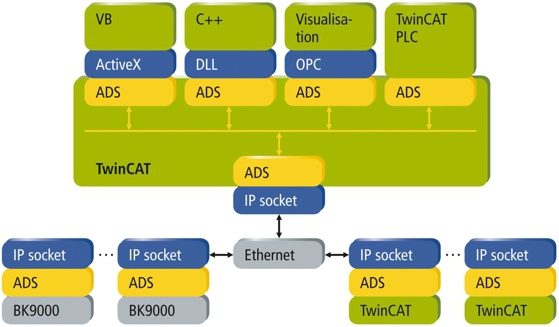
\includegraphics[width=0.8\textwidth]{../docs/assets/g2/ads_protocol.png}
\caption{Arquitectura del protocolo ADS: las aplicaciones cliente acceden a las variables del PLC a través del \emph{router} de TwinCAT. Fuente: Beckhoff Automation.}
\label{fig:ads}
\end{figure}

\subsection{Configuración previa en TwinCAT}

Para que Python pueda escribir en el IPC, del lado TwinCAT se debe:

\begin{enumerate}
  \item Declarar en una GVL llamada \texttt{VARIABLES} tres variables \texttt{BOOL}:
        \texttt{bRojo}, \texttt{bAzul}, \texttt{bAmarillo}.
  \item Configurar una \emph{route} ADS entre la PC y el IPC (AMS Net ID y puerto 851).
  \item Construir un \textbf{HMI} en TwinCAT con una \textbf{lámpara por color}, cada una
        enlazada a su variable \texttt{BOOL}, para verificar visualmente que el clasificador
        escribe la variable correcta.
\end{enumerate}

\subsection{La librería \texttt{pyads}}

El patrón básico de conexión y escritura se muestra en el Script~\ref{lst:pyads-basic}.
Los nombres en \texttt{write\_by\_name()} deben coincidir \emph{exactamente} con los de la
GVL (mayúsculas incluidas).

\begin{lstlisting}[language=Python, caption={Conexión y escritura básica con pyads.}, label={lst:pyads-basic}]
import pyads

ipc = pyads.Connection('192.168.57.231.1.1', 851)   # AMS Net ID del IPC
ipc.open()

ipc.write_by_name('VARIABLES.bRojo',     True,  pyads.PLCTYPE_BOOL)
ipc.write_by_name('VARIABLES.bAzul',     False, pyads.PLCTYPE_BOOL)
ipc.write_by_name('VARIABLES.bAmarillo', False, pyads.PLCTYPE_BOOL)

ipc.close()
\end{lstlisting}

% =============================================================================
\section{Integración: del clasificador a la acción del brazo}

El sistema opera bajo un contrato simple: el clasificador procesa el \emph{frame} de la
cámara y, si la confianza supera un umbral configurable (por defecto $0.6$), escribe
\texttt{True} en la variable del color predicho y \texttt{False} en las otras dos; si la
clase es \texttt{fondo} o la confianza es baja, las tres quedan en \texttt{False}. El PLC
detecta el flanco ascendente, activa la salida digital correspondiente y el brazo deposita
la tapita en su zona. El Script~\ref{lst:loop} integra captura, predicción y escritura ADS.

\begin{lstlisting}[language=Python, caption={Bucle principal: captura, predicción y escritura ADS.}, label={lst:loop}]
import cv2, numpy as np, pyads
from tensorflow.keras.models import load_model
from tensorflow.keras.applications.mobilenet_v2 import preprocess_input

UMBRAL = 0.6
IMG_SIZE = 128                                    # igual que al entrenar (NB4)
CLASES = ['amarillo', 'azul', 'fondo', 'rojo']    # orden alfabetico
VAR_POR_CLASE = {                                 # 'fondo' no activa ninguna salida
    'rojo': 'VARIABLES.bRojo',
    'azul': 'VARIABLES.bAzul',
    'amarillo': 'VARIABLES.bAmarillo',
}

modelo = load_model('modelo_tapitas.h5')
ipc = pyads.Connection('192.168.57.231.1.1', 851)
ipc.open()

cam = cv2.VideoCapture(0)
try:
    while True:
        ok, frame = cam.read()
        if not ok:
            break
        # Preprocesamiento MobileNetV2: BGR->RGB, resize y normalizar a [-1, 1]
        img = cv2.cvtColor(cv2.resize(frame, (IMG_SIZE, IMG_SIZE)), cv2.COLOR_BGR2RGB)
        x = np.expand_dims(preprocess_input(img.astype('float32')), axis=0)

        pred = modelo.predict(x, verbose=0)[0]
        idx = int(np.argmax(pred))
        clase, confianza = CLASES[idx], float(pred[idx])

        # Activa el BOOL del color detectado si supera el umbral; el resto en False.
        activo = VAR_POR_CLASE.get(clase) if confianza >= UMBRAL else None
        for var in VAR_POR_CLASE.values():
            ipc.write_by_name(var, var == activo, pyads.PLCTYPE_BOOL)

        cv2.putText(frame, f"{clase} ({confianza:.2f})", (10, 30),
                    cv2.FONT_HERSHEY_SIMPLEX, 0.8, (0, 255, 0), 2)
        cv2.imshow('Clasificador', frame)
        if cv2.waitKey(1) & 0xFF == ord('q'):
            break
finally:
    cam.release(); cv2.destroyAllWindows()
    for var in VAR_POR_CLASE.values():            # apagar todo al salir
        ipc.write_by_name(var, False, pyads.PLCTYPE_BOOL)
    ipc.close()
\end{lstlisting}

% =============================================================================
\section{Experiencia guiada}\label{sec:tl-practico}

La pareja ejecuta y completa los tres notebooks de la Parte~2 (igual que en la Parte~1:
ejecutar de principio a fin, completar las celdas marcadas y responder las preguntas). La
Parte~2 aporta \textbf{10 puntos}.

\renewcommand{\arraystretch}{1.35}
\begin{tabularx}{\textwidth}{@{}p{5.3cm} X r@{}}
\toprule
\textbf{Actividad (herramienta)} & \textbf{Qué se realiza} & \textbf{Puntos} \\
\midrule
1. Feature extraction \newline {\footnotesize(\texttt{notebook4}, secc. 2--6)}
  & Reutilizar el dataset de la Parte~1, construir el modelo con \emph{backbone} MobileNetV2 congelado, entrenar el cabezal y evaluar con curvas y matriz de confusión.
  & 3.0 \\
2. Fine-tuning \newline {\footnotesize(\texttt{notebook4}, secc. 4--5)}
  & Descongelar los últimos \emph{layers}, reentrenar con \emph{learning rate} pequeño y comparar contra la fase anterior y contra la CNN del Notebook~3.
  & 2.0 \\
3. Conexión ADS y HMI \newline {\footnotesize(TwinCAT + \texttt{pyads})}
  & Declarar las tres BOOL en la GVL, construir el HMI con una lámpara por color y escribirlas desde Python (Script~\ref{lst:pyads-basic}), verificando el encendido.
  & 2.0 \\
4. Demostración integrada \newline {\footnotesize(\texttt{notebook6} + brazo)}
  & Ejecutar el bucle de inferencia (Script~\ref{lst:loop}) con la cámara: cada color detectado activa su BOOL y dispara la acción del brazo. Grabar un video.
  & 2.5 \\
5. Discusión final
  & Reflexionar sobre cómo aplicar el sistema en el proyecto integrador de automatización.
  & 0.5 \\
\midrule
\textbf{Total Parte 2} & & \textbf{10.0} \\
\bottomrule
\end{tabularx}
\renewcommand{\arraystretch}{1}

% =============================================================================
\section{Anexos}

\subsection*{Anexo B1. Variables del proyecto TwinCAT}

\renewcommand{\arraystretch}{1.2}
\begin{tabularx}{\textwidth}{@{}p{3.0cm} p{2.0cm} X@{}}
\toprule
\textbf{Variable} & \textbf{Tipo} & \textbf{Descripción} \\
\midrule
\texttt{bRojo}     & \texttt{BOOL} & Verdadero al detectar una tapita roja sobre el umbral. \\
\texttt{bAzul}     & \texttt{BOOL} & Verdadero al detectar una tapita azul sobre el umbral. \\
\texttt{bAmarillo} & \texttt{BOOL} & Verdadero al detectar una tapita amarilla sobre el umbral. \\
\bottomrule
\end{tabularx}
\renewcommand{\arraystretch}{1}

Deben declararse dentro de la GVL \texttt{VARIABLES}; el nombre de la GVL forma parte del
identificador usado en \texttt{write\_by\_name()}.

\subsection*{Anexo B2. Diagnóstico de errores comunes}

\renewcommand{\arraystretch}{1.2}
\begin{tabularx}{\textwidth}{@{}p{5.5cm} X@{}}
\toprule
\textbf{Error} & \textbf{Causa y solución} \\
\midrule
\texttt{Missing ADS routes (7)} & Falta la \emph{route} ADS entre la PC y el IPC (\texttt{open()} no la valida; el error aparece al leer/escribir). Crearla en TwinCAT (bandeja) $\rightarrow$ Router $\rightarrow$ Edit Routes $\rightarrow$ Add Route. \\
\texttt{AdsError: symbol not found} & El nombre en \texttt{write\_by\_name} no coincide con la GVL. Verificar mayúsculas y el prefijo \texttt{VARIABLES.} \\
El brazo no se dispara & La variable se escribe pero el POU del PLC no actúa sobre ella. Verificar la lógica en TwinCAT. \\
Confianza alta pero clase incorrecta & Dataset poco diverso. Capturar más muestras en condiciones variadas. \\
\bottomrule
\end{tabularx}
\renewcommand{\arraystretch}{1}
